\section{Approach}
\label{s:approach}
%Approach; What selection of deep uncertainty methods are you using, in what order, and why? This should be clearly motivated and grounded in the literature

% Analysis is carried out across the explicated rival problem framings and relies on state-of- the-art deep uncertainty techniques

% Analysis is carried out across the explicated rival problem framings and relies on state-of- the-art deep uncertainty techniques
Multiple alternative approaches were considered to analyse the explicated problem framings. Ultimately, a straightforward combination of techniques were adopted to analyse and interpret the problem framings of Gorssel, as well as its two rival/coalition-forming actors, Deventer and Overijssel. A multi-scenario multi objective robust decision making (MORDM) process was chosen for the analysis and selection of policy approaches. This approach was selected for the ability to achieve a balance between finding robust solutions that are locally optimal in individual scenarios, while also being computationally efficient, given constraints in time and computing power \parencite{bartholomew_considering_2020}. A flow diagram for this approach is shown in Figure \ref{fig:msmordm}. Below, the deep uncertainty techniques applied in each of the steps are explained and selections of these approaches motivated in light of currently available literature. 

\begin{figure}[h]
    \centering
    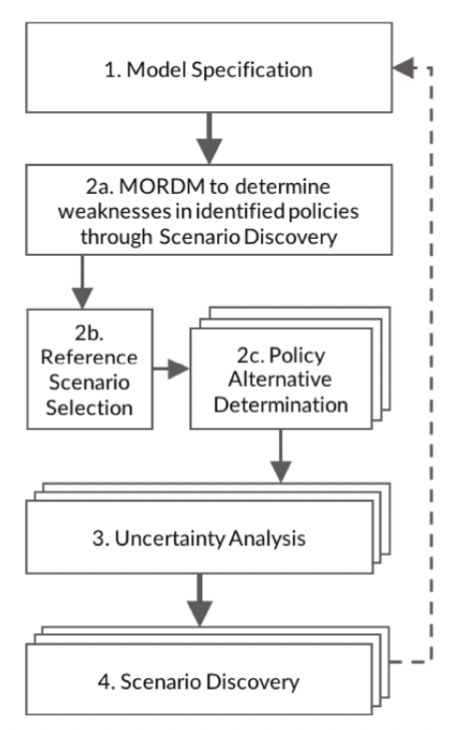
\includegraphics[width=0.4\textwidth]{report/figures/msmordm.png}
    \caption{The MSMORDM Process from \citeauthor{bartholomew_considering_2020}}
    \label{fig:msmordm}
\end{figure}

The Exploratory Modelling Workbench (an open source Python library) was used to implement this approach. Full details of the analysis implementation can be found in the repository in the appendix in Section \ref{s:reposit}.

%In what order are we using the tools and why are we using them this way
\subsection{Problem Formulation}
In the first step of this process, the problem formulations for each of the three actors were defined in the model, as described in Section \ref{s:prob_frame}. For each actor, multiple objectives were defined, to elicit relevant trade-offs (predominantly between cost and risk). These formulations were set to run across three planning steps, to observe evolution of planning and risk, and to get more granularity in the potential policies and uncertainties. The three actors were also formulated and run separately to reduce the dimensionality of the problem and to enable us to find preferred policies for each of the actors individually \parencite{trindade_reducing_2017}.

The underlying model was also modified to serve the selected problem formulation, by disaggregating the cost factors of Room for the River Costs and the Evacuations Costs, such that costs for the actors of Gorssel and Deventer were individualised.

\subsection{Preliminary MORDM}
Once the problem formulations for each actor were decided, a small round of MORDM was performed to identify ranges for uncertainties, over which multiple scenarios could be selected to perform complete multi-scenario MORDM. For this round, 50,000 scenarios were generated for each actor. We chose to run 50,000 scenarios for each actor in an effort to trade off the granularity/resolution of available scenarios against the computational intensity of generating and optimising over this large range. A large number of scenarios was also necessary as the chosen problem framing resulted in an increase in the number of uncertainties in the model (that is, the levers for actors outside of Overijssel Province).

Following scenario generation, policy alternatives were generated by optimising over the policy objectives for the three actors to determine the Pareto-approximate set, using a many-objective evolutionary algorithm. The algorithm used was $\epsilon$-NSGA2. This algorithm was considered appropriate for our formulations, as previous studies have shown that it performs well for six-objective problem formulations in related applications \parencite{salazar_diagnostic_2016}. The epsilon values for these optimisations were selected through a process of trial and error, informed by the range of values observed in the generated scenarios, with attention given to the number of potential policies generated from each iteration. We were ultimately satisfied that the chosen epsilon values represented an optimisation space which could trade-off between being able to generate a sufficient number of interesting policy combinations, without creating so much granularity that there was duplication or 'nonsense' policies being generated. The number of function evaluations for each optimisation were also selected based on trial and error, with the optimisations re-run until model results converged.

Following this, scenario discovery and feature scoring was conducted to identify the most important uncertainties in the model space for each of the three actors. Scenario discovery was conducted using the PRIM algorithm, as it allowed us to visualise and investigate the uncertainty space to identify suitable ranges of uncertainty for scenario selection in the multi-scenario MORDM process \parencite{bryant_thinking_2010}. This process revealed that the most important uncertainty for the three actors was the probability of dike failure at Gorssel. This factor was the strongest determinant of policy success across the widest range of scenarios.

With this information, we were then able to move to the next stage of analysis.

\begin{figure}[h]
    \centering
    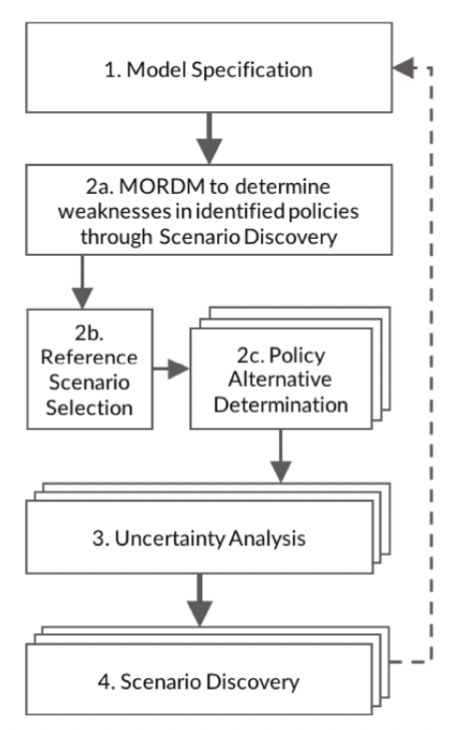
\includegraphics[width=0.4\textwidth]{report/figures/msmordm.png}
    \caption{The MSMORDM Process from \citeauthor{bartholomew_considering_2020}}
    \label{fig:msmordm}
\end{figure}


\subsection{Scenario Selection}
Provided this information on the importance of different uncertainties on outcomes of interest, we developed a process for selection of six scenarios, over which policies could be generated and optimised. Attention was given to ensure a good distribution of dike failure probability values across the selected scenarios. We opted for a mixture of good, 'middle' and worst case scenarios, to enable us to observe performance of and preferences towards policies under the widest range of scenarios. This was also done to support stakeholder comprehension of policy outcomes. The two 'worst case' scenarios (one representing worst case for deaths, and another across all outcomes) exist within the uncertainty range for probability of failure identified in the previous step. This approach was selected instead of a 'maximise diversity' approach due to time constraints in the computational intensity of such an approach over such a large number of scenarios and uncertainties \parencite{eker_including_2018}.

\subsection{Identifying Policy Alternatives}
Having selected these six scenarios over which to optimise, the MOEA was run again (as in the preliminary MORDM step) to identify Pareto-approximate policies for each of the scenarios, for each actor. Following this optimisation, KMeans clustering was used to select a more manageable subset of \textcolor{red}{five} appropriately robust policies for each actor were chosen for further robustness analysis.  This sub-setting was necessary due to time constraints.



\subsection{Robustness Analysis}
The subsetted selection of policy alternatives were then examine in terms of their robustness according to two types of robustness metrics: one satisficing, and one regret based. The use of two metrics was deemed necessary to see where there might be disagreement between the two types of metrics, and to identify if any policies achieve good scores under both metrics (indicating  policies that are more robust across different perspectives) \parencite{mcphail_robustness_2018}. These robustness metrics then resulted in a final shortlist of five candidate policies per actor.

The threshold values for the satisficing analysis can be found in \autoref{tab:threshold}. The threshold values for the total costs are the exact budgets of the institutions for water/traffic management so that it is a somewhat realistic representation. Expected annual damage was taken as 10\% of the Total costs that are available every year to the institutions. The values for expected annual casualties is calculated from the maximum risk of 1:100,000 people that can die from flooding multiplied \parencite{slootjes_achtergronden_2016} . Which is then multiplied with the amount of inhabitants of the area.


\begin{table}[H]
\centering
\caption{This table shows the threshold values for the three actors. The values for the town of Gorssel come from its bigger municipality Lochem \parencite{gorssel-2021}. Deventer's value is derived from \parencite{deventer-2021}. The value for Overijssel is gained from \parencite{provincie-overijssel-2021}.}
\label{tab:threshold}
\begin{tabular}{@{}llll@{}}
\cmidrule(l){2-4}
 &
  \multicolumn{3}{c}{\textbf{Robustness threshold values}} \\ \cmidrule(l){2-4} 
\multicolumn{1}{l|}{} &
  \multicolumn{1}{l|}{\textbf{Outcome}} &
  \multicolumn{1}{l|}{\textbf{Goal}} &
  \multicolumn{1}{l|}{\textbf{Threshold}} \\ \cmidrule(l){2-4} 
\multicolumn{1}{c|}{\multirow{3}{*}{Gorssel}} &
  \multicolumn{1}{l|}{\begin{tabular}[c]{@{}l@{}}Expected annual\\ damage\end{tabular}} &
  \multicolumn{1}{l|}{Minimize} &
  \multicolumn{1}{l|}{$5.4E+05$} \\ \cmidrule(l){2-4} 
\multicolumn{1}{c|}{} &
  \multicolumn{1}{l|}{\begin{tabular}[c]{@{}l@{}}Expected annual\\ casualties\end{tabular}} &
  \multicolumn{1}{l|}{Minimize} &
  \multicolumn{1}{l|}{$1.0E-05$} \\ \cmidrule(l){2-4} 
\multicolumn{1}{c|}{} &
  \multicolumn{1}{l|}{Total costs} &
  \multicolumn{1}{l|}{Minimize} &
  \multicolumn{1}{l|}{$5.4E+06$} \\ \cmidrule(l){2-4} 
\multicolumn{4}{l}{} \\ \cmidrule(l){2-4} 
\multicolumn{1}{l|}{\multirow{3}{*}{Deventer}} &
  \multicolumn{1}{l|}{\begin{tabular}[c]{@{}l@{}}Expected annual\\ damage\end{tabular}} &
  \multicolumn{1}{l|}{Minimize} &
  \multicolumn{1}{l|}{$1.1E+06$} \\ \cmidrule(l){2-4} 
\multicolumn{1}{l|}{} &
  \multicolumn{1}{l|}{\begin{tabular}[c]{@{}l@{}}Expected annual\\ casualties\end{tabular}} &
  \multicolumn{1}{l|}{Minimize} &
  \multicolumn{1}{l|}{$1.0E-05$} \\ \cmidrule(l){2-4} 
\multicolumn{1}{l|}{} &
  \multicolumn{1}{l|}{Total costs} &
  \multicolumn{1}{l|}{Minimize} &
  \multicolumn{1}{l|}{$1.1E+07$} \\ \cmidrule(l){2-4} 
\multicolumn{4}{l}{} \\ \cmidrule(l){2-4} 
\multicolumn{1}{l|}{\multirow{3}{*}{Overijssel}} &
  \multicolumn{1}{l|}{\begin{tabular}[c]{@{}l@{}}Expected annual\\ damage\end{tabular}} &
  \multicolumn{1}{l|}{Minimize} &
  \multicolumn{1}{l|}{$1.53E+06$} \\ \cmidrule(l){2-4} 
\multicolumn{1}{l|}{} &
  \multicolumn{1}{l|}{\begin{tabular}[c]{@{}l@{}}Expected annual\\ casualties\end{tabular}} &
  \multicolumn{1}{l|}{Minimize} &
  \multicolumn{1}{l|}{$1.0E-05$} \\ \cmidrule(l){2-4} 
\multicolumn{1}{l|}{} &
  \multicolumn{1}{l|}{Total costs} &
  \multicolumn{1}{l|}{Minimize} &
  \multicolumn{1}{l|}{$1.53E+07$} \\ \cmidrule(l){2-4} 
\end{tabular}
\end{table}

\subsection{Uncertainty Analysis and Scenario Discovery}
Here, a similar process was taken as in the preliminary MORDM to identify uncertainty spaces and tradeoffs between outcomes for each actor, this time performed over a larger array of policies and scenarios. The outcomes of this analysis will inform future iterations over the MORDM process, and reformulations of the uncertainty space, objectives, and (potentially) the levers available to the actors.

\subsection{Sensitivity Analysis}
The candidate policies for each actor where then assessed for their sensitivity to input factors. The chosen method for global sensitivity analysis was the Extra Trees algorithm. This approach was chosen, as it is known to be an effective means of replicating the insights of a global sensitivity analysis with much lower computational requirements \parencite{jaxa-rozen_tree-based_2018}.

\subsection{Policy Synthesis}
Finally, we identified where there are policies that are consistent (or at least similar) between actors to support coalition forming (in the case of consistent policies) or informing policy negotiations (in the case of inconsistent policies). The five candidate policies from each actor were compared to find potential similarities in lever choices, which go to informing opportunities for coalition-building or areas for negotiation in further formulations and iterations over the MORDM process.



